\chapter{Протокол ИРБИС64}

\section{Инструментарий для исследования протокола}

Удобным инструментом для изучения протокола ИРБИС64 является бесплатный анализатор сетевого трафика Wireshark (https://www.wireshark.org/): 

1. Скачиваем и устанавливаем WireShark, включаем в нём фильтр "tcp.port == 6666", чтобы отсечь лишний трафик. 

2. Пусть мы хотим изучить часть протокола, относящуюся к сохранению записи на сервере. Тогда захват пакетов мы должны включить непосредственно перед изучаемой операцией и выключать сразу после её выполнения, иначе придётся будет захвачено через множество число пакетов, не относящихся к делу. 

3. Отыскиваем нужный пакет (в данном случае "D" - сохранение записи) (см. рис. \ref{wireshark}). Видно, что в нём 1156 байт данных, из них 4 - длина пакета и перевод строки \\x0A.

\begin{figure}[h]
	\centering
	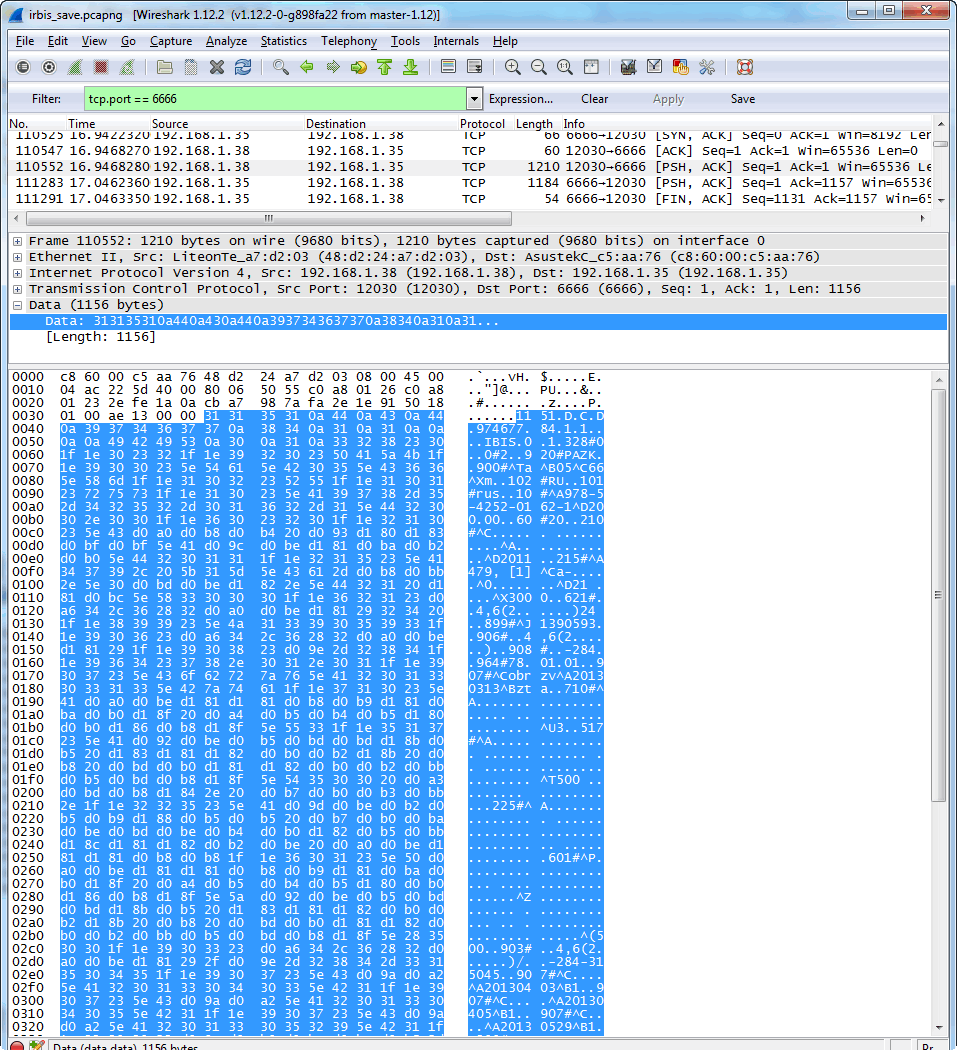
\includegraphics[width=0.7\textwidth]{wireshark}
	\caption{Окно Wireshark с захваченным сетевым пакетом} \label{wireshark}
\end{figure}

Вот пример пакета с запросом АРМ "Каталогизатор" (рис. \ref{dump1}):

\begin{figure}[h]	
	\centering
	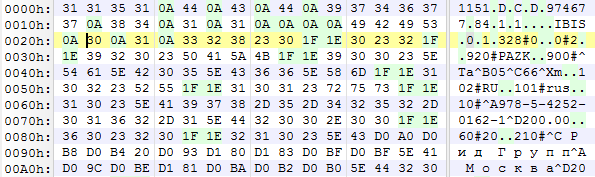
\includegraphics[width=0.7\textwidth]{dump1}
	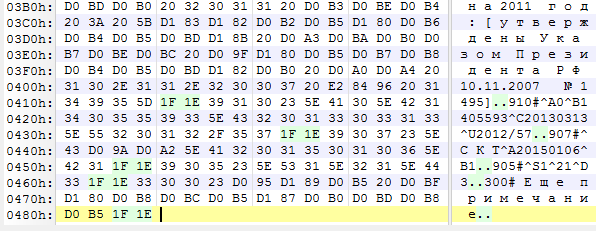
\includegraphics[width=0.7\textwidth]{dump2}
	\caption{Запрос клиента (часть информации опущена)} \label{dump1}
\end{figure}

\begin{table}[htbp]
	\centering
	\caption{Запрос клиента}
	\begin{tabular}{ | p{0.3\textwidth} | p{0.3\textwidth} | p{0.3\textwidth} | }
		\hline
		\textbf{Данные} & 
		\textbf{Назначение} &
		\textbf{Примечания}
		\\ \hline
		\hline
		\textbf{1150} &
		общая длина пакета в байтах &
		кодировка ANSI, перевод строки 0x0A		
		\\ \hline
		\textbf{D} &
		код команды &
		\\ \hline
		\textbf{C} &
		код АРМ "Каталогизатор" &
		\\ \hline
		\textbf{D} &
		код команды (повторение) &
		\\ \hline
		\textbf{974677} &
		идентификатор клиента &
		\\ \hline
		\textbf{84} &
		порядковый номер команды &
		\\ \hline
		\textbf{1} &
		пароль &
		\\ \hline
		\textbf{1} &
		логин &
		\\ \hline
		& пустая строка &
		\\ \hline
		& пустая строка &
		\\ \hline
		& пустая строка &
		\\ \hline
		\textbf{IBIS} &
		имя базы данных &
		\\ \hline
		\textbf{0} &
		признак (не)блокировки записи &
		\\ \hline
		\textbf{1} &
		признак актуализации &
		\\ \hline
		328\#0 &
		MFN записи и ее статус &
		кодировка UTF8, перевод строки 0x01F 0x1E
		\\ \hline
		0\#2 &
		0 и версия записи &
		\\ \hline
		920\#PAZK &
		начало полей записи &
		\\ \hline
		\dots &
		поля записи &
		\\ \hline
		330\#Ещё примечание &
		последнее поле записи, заканчивается переводом строки 0x1F 0x1E &
		\\ \hline
	\end{tabular}
\end{table}

Теперь пакет с ответом сервера (рис. \ref{dump3}):

\begin{figure}[h]	
	\centering
	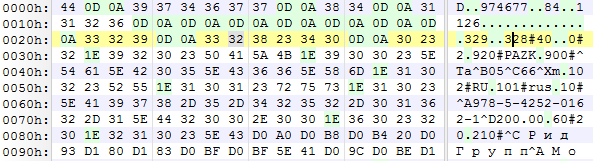
\includegraphics[width=0.7\textwidth]{dump3}
	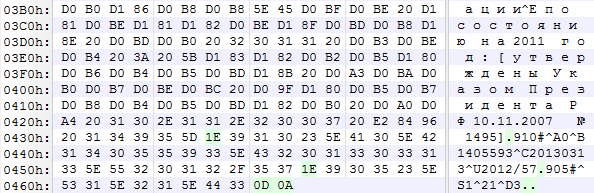
\includegraphics[width=0.7\textwidth]{dump4}
	\caption{Ответ сервера (часть информации опущена)} \label{dump3}
\end{figure}

\section{Команды протокола ИРБИС64}

\begin{table}[htbp]
	\centering
	\caption{Команды протокола}
	\begin{tabular}{ | p{0.07\textwidth} | p{0.43\textwidth} | p{0.2\textwidth} |  p{0.2\textwidth} | }
		\hline
		\textbf{Код} & \textbf{Команда} & \textbf{Реализована} & \textbf{Примечания}
		\\ \hline
		\hline
		\textbf{\#} & Получение признака монопольной блокировки базы данных & & ??? \\
		\hline
		\textbf{0} & Получение списка удаленных, неактуализированных, блокированных записей и статуса блокировки базы данных & + & \\
		\hline
		\textbf{1} & Получение версии сервера & + & Начиная с 2008.1 \\
		\hline
		\textbf{2} & Получение статистики по базе данных & & \\
		\hline
		\textbf{3} & IRBIS\_FORMAT\_ISO\_GROUP & & ??? \\
		\hline
		\textbf{4} & ??? & & \\
		\hline
		\textbf{5} & Глобальная корректировка & & \\
		\hline
		\textbf{6} & Сохранение группы записей & + & \\
		\hline
		7 & Печать & & \\
		\hline
	\end{tabular}
\end{table}

